\section{相关平均的方差}
\label{sec:mcerr-correlated}

上一节处理的是链平均的偏差，现在把它放在一边，假定链从$\pi$出发，于是$\hat{I}_N$无偏，误差只剩随机波动。链的相邻状态相关，式~\eqref{eq:mcerr-iid-var}的推导用到了独立性，不能照搬。相关性究竟让波动变大还是变小，变多少？先对固定的$N$精确计算方差，再看$N$很大时它的主要部分。

\subsection{平稳平均的方差}
\label{sec:mcerr-stationary-var}

设链平稳，$\mathbb{E}_{\pi}[f^{2}]<\infty$。对任意时刻$s$，$X^{(s)}\sim\pi$，并且从$X^{(s)}$往后按同一个核演化，所以$(X^{(s)},X^{(s+k)})$与$(X^{(0)},X^{(k)})$有相同的联合分布。于是两时刻函数值的协方差只依赖时间差$k$，记
\begin{equation}
 \gamma_k=\operatorname{Cov}_{\pi}\bigl(f(X^{(0)}),f(X^{(k)})\bigr),\qquad k=0,1,2,\dots
 \label{eq:mcerr-autocov}
\end{equation}
它称为$f$沿链的\term{自协方差}（autocovariance）。$\gamma_0=\operatorname{Var}_{\pi}(f)$，由Cauchy--Schwarz不等式，$\lvert\gamma_k\rvert\leq\gamma_0$。

\begin{theorem}[平稳平均的方差]
\label{thm:mcerr-stationary-var}
设链平稳，$\mathbb{E}_{\pi}[f^{2}]<\infty$。则对每个$N\geq1$，
\begin{equation}
 \operatorname{Var}(\hat{I}_N)=\frac1N\Bigl[\gamma_0+2\sum_{k=1}^{N-1}\Bigl(1-\frac{k}{N}\Bigr)\gamma_k\Bigr] .
 \label{eq:mcerr-stationary-var}
\end{equation}
\end{theorem}

\begin{proof}
记$Y_t=f(X^{(t)})$。和的方差等于全部协方差之和，
\[
 \operatorname{Var}\Bigl(\sum_{t=1}^{N}Y_t\Bigr)=\sum_{s=1}^{N}\sum_{t=1}^{N}\operatorname{Cov}(Y_s,Y_t)=\sum_{s=1}^{N}\sum_{t=1}^{N}\gamma_{\lvert s-t\rvert} .
\]
在$N\times N$的下标方阵中，$\lvert s-t\rvert=0$的格子有$N$个（对角线）；对$1\leq k\leq N-1$，$\lvert s-t\rvert=k$的格子在对角线两侧各有$N-k$个。按$k$合并，
\[
 \operatorname{Var}\Bigl(\sum_{t=1}^{N}Y_t\Bigr)=N\gamma_0+2\sum_{k=1}^{N-1}(N-k)\gamma_k .
\]
两边除以$N^{2}$即得。
\end{proof}

与独立情形比较，式~\eqref{eq:mcerr-stationary-var}多了方括号里的求和。各$\gamma_k$为正时，方差大于$\gamma_0/N$：相邻状态差不多，第二个样本带来的新信息少于一个独立样本，好比反复询问同一户人家。各$\gamma_k$正负交替时，方差可以小于$\gamma_0/N$：相邻状态落在两侧，平均时互相抵消。所以链输出的方差既可能比独立平均大，也可能比它小；直接把$S_N^{2}/N$当作链平均的方差，没有任何依据。

\paragraph{例子中的自协方差}
对链~\eqref{eq:mcerr-ar1}与$f(x)=x$，$X^{(k)}$等于$\rho^{k}X^{(0)}$加上一个与$X^{(0)}$独立的项，所以
\[
 \gamma_k=\operatorname{Cov}\bigl(X^{(0)},\rho^{k}X^{(0)}\bigr)=\rho^{k} .
\]
对$f(x)=x^{2}$，记$Z$为与$X^{(0)}$独立的标准正态变量，$X^{(k)}=\rho^{k}X^{(0)}+\sqrt{1-\rho^{2k}}\,Z$，平方后
\[
 (X^{(k)})^{2}=\rho^{2k}(X^{(0)})^{2}+2\rho^{k}\sqrt{1-\rho^{2k}}\,X^{(0)}Z+(1-\rho^{2k})Z^{2} .
\]
与$(X^{(0)})^{2}$求协方差时，第二项的协方差是$\mathbb{E}[(X^{(0)})^{3}]\,\mathbb{E}[Z]=0$，第三项与$X^{(0)}$独立，只剩第一项。标准正态变量平方的方差是$2$，所以$\gamma_k=2\rho^{2k}$。

\paragraph{四步的平均}
取$N=4$，$f(x)=x$。$\rho=0.9$时，由式~\eqref{eq:mcerr-stationary-var}，
\[
 \operatorname{Var}(\hat{I}_4)=\frac14\bigl[1+2(0.75\times0.9+0.5\times0.81+0.25\times0.729)\bigr]=\frac{3.5245}{4}=0.8811 .
\]
$\rho=-0.5$时，
\[
 \operatorname{Var}(\hat{I}_4)=\frac14\bigl[1+2(-0.75\times0.5+0.5\times0.25-0.25\times0.125)\bigr]=\frac{0.4375}{4}=0.1094 .
\]
同样长度的独立平均方差是$0.25$。正相关的链把方差放大到约$3.5$倍，负相关的链把它缩小到约$0.44$倍。

图~\ref{fig:mcerr-ar-paths}用同一串噪声画出三条平稳链。$\rho=0.9$的路径缓慢起伏，$80$步的平均为$0.45$；$\rho=0$即独立样本，平均为$0.097$；$\rho=-0.5$的路径在$0$两侧来回跳，平均只有$0.055$。图~\ref{fig:mcerr-autocov}(a)画出两种$\rho$下的$\gamma_k$。

\begin{BookInlineFigure}
 \centering
 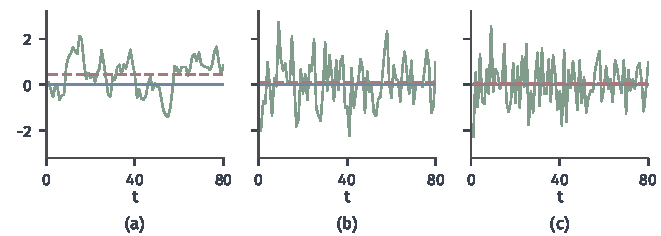
\includegraphics[width=112mm]{figures/07-probability/08-sampling-and-integration/matplotlib/mcerr-ar-paths/figure.pdf}
 \caption{平稳链~\eqref{eq:mcerr-ar1}的$80$步路径（绿线），三图使用同一串噪声与初值（种子$3129$）。(a)$\rho=0.9$；(b)$\rho=0$；(c)$\rho=-0.5$。蓝线为$I=0$，红色虚线为$80$步的平均。}
 \label{fig:mcerr-ar-paths}
\end{BookInlineFigure}

\subsection{长期方差}
\label{sec:mcerr-long-run}

链平均的方差公式~\eqref{eq:mcerr-stationary-var}含有$N$个项，比较两条链或两个被积函数时不方便。$N$很大时，权重$1-k/N$对固定的$k$趋于$1$，方括号趋于一个与$N$无关的数，它就是比较精度时需要的量。

\begin{definition}[长期方差]
\label{def:mcerr-long-run}
设链平稳，$\mathbb{E}_{\pi}[f^{2}]<\infty$，且$\sum_{k\geq1}\lvert\gamma_k\rvert<\infty$。称
\begin{equation}
 \sigma_{\mathrm{LR}}^{2}=\gamma_0+2\sum_{k=1}^{\infty}\gamma_k
 \label{eq:mcerr-long-run}
\end{equation}
为$f$沿链的\term{长期方差}（long-run variance）。
\end{definition}

\begin{theorem}[方差的极限]
\label{thm:mcerr-long-run-limit}
在定义~\ref{def:mcerr-long-run}的条件下，
\begin{equation}
 \lim_{N\to\infty}N\operatorname{Var}(\hat{I}_N)=\sigma_{\mathrm{LR}}^{2} .
 \label{eq:mcerr-nvar-limit}
\end{equation}
\end{theorem}

\begin{proof}
由式~\eqref{eq:mcerr-stationary-var}与式~\eqref{eq:mcerr-long-run}，
\[
 N\operatorname{Var}(\hat{I}_N)-\sigma_{\mathrm{LR}}^{2}=-2\sum_{k=N}^{\infty}\gamma_k-2\sum_{k=1}^{N-1}\frac{k}{N}\gamma_k .
\]
第一项是收敛级数的尾部，趋于零。第二项中第$k$项$(k/N)\gamma_k\mathbf{1}_{\{k<N\}}$的绝对值不超过$\lvert\gamma_k\rvert$，而且对固定的$k$，它随$N\to\infty$趋于零。$\lvert\gamma_k\rvert$可和，由支配收敛定理（用于计数测度上的级数），第二项也趋于零。
\end{proof}

于是$N$大时$\operatorname{Var}(\hat{I}_N)\approx\sigma_{\mathrm{LR}}^{2}/N$，链平均仍按$N^{-1/2}$收缩，只是把独立情形的$\gamma_0$换成了$\sigma_{\mathrm{LR}}^{2}$。对链~\eqref{eq:mcerr-ar1}与$f(x)=x$，
\[
 \sigma_{\mathrm{LR}}^{2}=1+2\sum_{k=1}^{\infty}\rho^{k}=1+\frac{2\rho}{1-\rho}=\frac{1+\rho}{1-\rho} .
\]
$\rho=0.9$时为$19$，$\rho=-0.5$时为$1/3$。图~\ref{fig:mcerr-autocov}(b)画出$N\operatorname{Var}(\hat{I}_N)$的精确值：$\rho=0.9$时，$N=4$为$3.52$，$N=100$为$17.20$，$N=1000$为$18.82$，逐步接近$19$。接近的快慢由$\gamma_k$衰减的快慢决定。

\begin{BookInlineFigure}
 \centering
 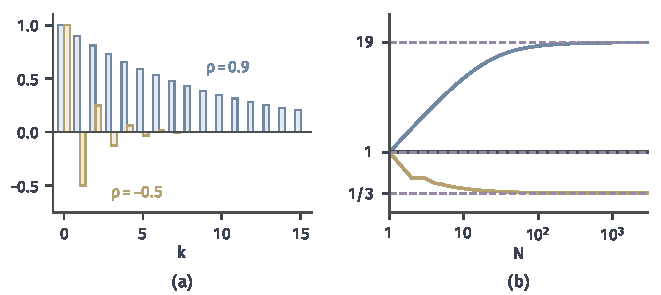
\includegraphics[width=112mm]{figures/07-probability/08-sampling-and-integration/matplotlib/mcerr-autocov/figure.pdf}
 \caption{平稳链~\eqref{eq:mcerr-ar1}与$f(x)=x$。(a)自协方差$\gamma_k=\rho^{k}$，蓝色为$\rho=0.9$，黄色为$\rho=-0.5$；(b)由式~\eqref{eq:mcerr-stationary-var}算出的$N\operatorname{Var}(\hat{I}_N)$，蓝、灰、黄线分别对应$\rho=0.9,0,-0.5$，紫色虚线为长期方差$19,1,1/3$，双对数坐标。}
 \label{fig:mcerr-autocov}
\end{BookInlineFigure}

\paragraph{可和条件不成立时}
协方差不可和时，方差的极限可以不存在。考虑状态空间$\{0,1\}$上始终停在原地的链，从$\pi=(1/2,1/2)$出发，取$f$为状态$1$的示性函数。每一步的状态都等于$X^{(0)}$，所以$\gamma_k=1/4$对所有$k$成立，级数发散；实际上$\hat{I}_N=f(X^{(0)})$，$\operatorname{Var}(\hat{I}_N)=1/4$根本不随$N$缩小，$N\operatorname{Var}(\hat{I}_N)\to\infty$。

\paragraph{方差极限不是正态极限}
定理~\ref{thm:mcerr-long-run-limit}只说明了二阶矩的尺度，没有说$\sqrt{N}(\hat{I}_N-I)$的分布趋于正态。独立情形下这一步由中心极限定理完成，链的情形还需要关于链与$f$的附加条件，第~\ref{sec:mcerr-chain-clt}小节会给出一个满足可和条件、极限却不是正态的例子。

\subsection{有效样本量}
\label{sec:mcerr-ess}

长期方差告诉我们链平均的方差约为$\sigma_{\mathrm{LR}}^{2}/N$。把它与同样被积函数的独立平均$\gamma_0/N$比较，可以换算成“相当于多少个独立样本”。

\begin{definition}[有效样本量]
\label{def:mcerr-ess}
在定义~\ref{def:mcerr-long-run}的条件下，设$0<\gamma_0<\infty$，$0<\sigma_{\mathrm{LR}}^{2}<\infty$。长度为$N$的平稳链平均的\term{有效样本量}（effective sample size）为
\begin{equation}
 N_{\mathrm{eff}}=\frac{N\gamma_0}{\sigma_{\mathrm{LR}}^{2}} .
 \label{eq:mcerr-ess}
\end{equation}
\end{definition}

由式~\eqref{eq:mcerr-nvar-limit}，$\operatorname{Var}(\hat{I}_N)\approx\gamma_0/N_{\mathrm{eff}}$，即链平均与$N_{\mathrm{eff}}$个独立样本的平均有相同的渐近方差。表~\ref{tab:mcerr-ess}列出链~\eqref{eq:mcerr-ar1}上两个被积函数的$N_{\mathrm{eff}}/N$。$f(x)=x^{2}$的长期方差由$\gamma_k=2\rho^{2k}$求和得到：
\[
 \sigma_{\mathrm{LR}}^{2}=2+4\sum_{k=1}^{\infty}\rho^{2k}=\frac{2(1+\rho^{2})}{1-\rho^{2}} .
\]

\begin{BookInlineTable}
 \centering
 \caption{链~\eqref{eq:mcerr-ar1}上两个被积函数的长期方差与有效样本量}
 \label{tab:mcerr-ess}
 \begin{tabular}{lcccc}
  \toprule
  & \multicolumn{2}{c}{$\rho=0.9$} & \multicolumn{2}{c}{$\rho=-0.5$} \\
  & $\sigma_{\mathrm{LR}}^{2}$ & $N_{\mathrm{eff}}/N$ & $\sigma_{\mathrm{LR}}^{2}$ & $N_{\mathrm{eff}}/N$ \\
  \midrule
  $f(x)=x$，$\gamma_0=1$ & $19$ & $0.053$ & $1/3$ & $3$ \\
  $f(x)=x^{2}$，$\gamma_0=2$ & $19.05$ & $0.105$ & $10/3$ & $0.6$ \\
  \bottomrule
 \end{tabular}
\end{BookInlineTable}

这张表说明了有效样本量的几个特点。

第一，它依赖被积函数。同一条$\rho=-0.5$的链，估计均值时一个状态顶三个独立样本，估计二阶矩时只顶$0.6$个：$f(x)=x$的自协方差正负交替，平方以后$\gamma_k=2\rho^{2k}$全为正。$\rho=0.9$时两者也相差一倍。所以说“这条链的有效样本量”而不指明$f$是不完整的。

第二，它可以超过$N$。负相关时$\sigma_{\mathrm{LR}}^{2}<\gamma_0$，$N_{\mathrm{eff}}>N$。因此它不是记录中“真正独立的样本”的个数，只是渐近方差的一种换算。

第三，它需要估计。实际中$\gamma_0$与$\sigma_{\mathrm{LR}}^{2}$都未知，要从记录中估计，估计误差会直接传给$N_{\mathrm{eff}}$，下一节讨论怎样估计长期方差。

第四，它不能证明链已收敛。有效样本量是在链平稳的前提下定义的，用记录估计时，它反映的是链在已到过区域内的相关程度。一条被困在目标局部的链，可以有很大的估计有效样本量，第~\ref{sec:mcerr-diagnostics}小节会看到这样的例子。
